\documentclass[a4paper,10pt]{article}
\usepackage[utf8]{inputenc}
\usepackage{amsmath}
\usepackage{amsfonts}
\usepackage{amssymb}
\usepackage{makeidx}
\usepackage[a4paper,margin=2.5cm]{geometry}
\usepackage{verbatim}
\author{Quentin DEXHEIMER}
\usepackage{graphicx}
\usepackage{listings}
\title{Rapport Puppet - Part.3}

\begin{document}
	\section{Le travail réalisé}
		\subsection{Le script de réservation.}
Nous avons réalisé un script qui nous permet de reserver des machines sans avoir à renseigner les commandes de l'outil OAR. Nous demandons à la personne souhaitant réserver des machines de rentrer le nom de la réservation, le nombre de machines et le temps de réservation de celles-ci. Nous passons ensuite ces arguments à oarsub avec les options requises.
			
		\begin{figure}[!h]
			\centering
			\begin{verbatim}
			oarsub -I -t deploy -l {"type='kavlan-local'"}/vlan=1+/nodes=$nbr_nodes,
			walltime=$tmps -n "$nom"
			\end{verbatim}			
			\caption{La commande que nous passons en paramètre.}
		\end{figure}
		
		\subsection{Le script d'installation sur les machines.}
		Ce script nous permet d'automatiser l'installation de notre cluster une fois les machines réservées.
		\\
	Nous commençons l'installation de notre cluster par l'activation du DHCP de Grid5000.
		\\
	Nous installons ensuite une gem Ruby pour configurer et installer le service DHCP du VLAN qui nous concerne, configuré avec notre configuration de machines.
		\begin{figure}[!h]
			\centering
			\begin{verbatim}
			##Activation du DHCP g5k
kavlan -e
##Récupération du numéro VLAN
jobid=`oarstat | grep $USER | cut -d' ' -f1`
vlan=`kavlan -V -j $jobid `
site=`uname -n | cut -d"." -f2`
##Génération du fichier de configuration du DHCP
export GEM_HOME=/home/$USER/.gem/ruby/1.8/
gem install ruby-ip --no-ri --no-rdoc --user-install #&>/dev/null
chmod +x ./projet/install/gen_dhcpd_conf.rb #&>/dev/null
./projet/install/gen_dhcpd_conf.rb --site $site --vlan-id $vlan #&>/dev/null
mv dhcpd-kavlan-$vlan-$site.conf $puppet_modules/dhcp/files/dhcpd.conf

			\end{verbatim}			
			\caption{On active le DHCP du Grid5000 pour créer notre fichier de configuration, qui servira pour notre propre service DHCP.}
		\end{figure}
		Nous allons ensuite déployer l'image ISO de Debian que nous fournit le Grid5000 pour installer les différents services sur les noeuds. Nous affichons auparavant la liste des noeuds que nous avons réservés, avec le suffixe du vlan.
		\begin{figure}[!h]
			\centering
			\begin{verbatim}		 
					 
echo "-=-=-"
echo "Déploiement de l'environnement Linux, Debian Squeeze 64bit,
sur toutes les machines réservées (Peut prendre plusieurs minutes)."
kadeploy3 -e squeeze-x64-base -f $OAR_FILE_NODES 
--vlan $vlan -d -V4 -k $HOME/.ssh/id_dsa.pub &>/dev/null
echo "-=-=-"		 
			\end{verbatim}
			\caption{On utilise la commande kadeploy3 pour déployer toutes nos machines sous Debian Squeeze.}
			\label{kadeploy3}
		\end{figure}
		
		Vient ensuite l'ensemble des tests sur la configuration SSH du client qui a lancé le déploiement. Cela consiste en une vérification sur le fichier de configuration et le fichier authorized\_keys, puis en une copie des clés de l'utilisateur sur toutes les machines concernées par le déploiement du cluster.
		
		\begin{figure}[!h]
			\centering
			\begin{verbatim}			 
taktuk -l root -s -m $node broadcast exec [ 'cat ~/.ssh/id_dsa.pub 
>> ~/.ssh/authorized_keys' ]	
			\end{verbatim}
			\caption{Taktuk nous permet de réaliser l'insertion de la clé publique SSH dans le fichier authorized\_keys à distance.}
			\label{taktuk}
		\end{figure}
		Nous créons ensuite les tunnels SSH et nous mettons à jour tous les dépôts. Cela nous permet d'installer 
ensuite le master puppet et de lui spécifier tous les clients qui vont recevoir des services réseau.		
		\begin{figure}[!h]
			\centering
			\begin{verbatim}			 
echo "Attribution des rôles effectués:"
echo "- "`sed -n '2 p' $puppet_clients `" : dhcp,"
echo "- "`sed -n '3 p' $puppet_clients `" : bind,"
echo "- "`sed -n '4 p' $puppet_clients `" : mysql,"
echo "- "`sed -n '5 p' $puppet_clients `" : nfs,"
echo "- "`sed -n '6 p' $puppet_clients `" : oar-server,"
echo "- "`sed -n '7 p' $puppet_clients `" : oar-frontend,"
echo "- "`sed -n '8 p' $puppet_clients `" : kadeploy." 
			\end{verbatim}
			\caption{On définit quel noeud va recevoir quel service, de manière à ce que le master puppet n'installe pas tout sur la m\^eme machine.}
			\label{installPuppet}
		\end{figure}
		Une fois le ma\^itre configuré, nous installons et nous configurons tous nos clients de telle sorte que chaque machine puisse recevoir la configuration qui lui est attribuée depuis le master.
		
		Enfin, nous terminons l'installation par la désactivation du vlan fourni par Grid5000 pour utiliser notre propre serveur DHCP, puis par la suppression du fichier temporaire utilisé.		
		\begin{figure}[!h]
			\centering
			\begin{verbatim}			 
taktuk -l root -s -f $puppet_clients broadcast exec [ dhclient ] &>/dev/null
taktuk -l root -s -f $list_users broadcast exec [ dhclient ] &>/dev/null
rm lol.tmp		
			\end{verbatim}
			\caption{Fin du déploiement.}
			\label{fin}
		\end{figure}	
		
		\subsection{Le script de configuration du serveur.}
		Ce script permet d'écrire toute la configuration du maître Puppet en se basant sur tous les services à  installer. Pour commencer, nous configurons le fichier /etc/hostname pour établir le nom du réseau. Nous redémarrons ensuite le service de noms d'hôte.
		Nous ajoutons ensuite dans le fichier de configuration de Puppet le nom du serveur maître, car notre master puppet est aussi un agent. A cela se greffe une section contenant le nom de la machine qui validera les certificats, en l'occurence la machine maître, le tout placé dans une section.
		Nous avons également besoin de configurer les adresses ou les noms de nos machines clientes pour que Puppet puisse les retrouver. 		
		\begin{figure}[!h]
			\centering
			\begin{verbatim}			#ajout des hosts clients
y=1
for role in "puppet" "dhcp" "dns" "mysql" "nfs" "oar-frontend" "oar-server" "kadeploy"
do
	node=`sed -n $y"p" puppet_clients`
	ip_node=`arp $node | cut -d" " -f2 | cut -d"(" -f2 | cut -d")" -f1`
	echo "$ip_node $role.ptut-grid5000.lan" >> /etc/hosts
	y=$(($y+1))
done
			\end{verbatim}
			\caption{L'ajout des machines se fait à l'aide d'une boucle.}
			\label{Ajout Machines dans nodes.pp}
		\end{figure}
	
	Nous utilisons le m\^eme type de boucle pour définir les noeuds dans le fichier nodes.pp.
		 Enfin, nous terminons la configuration du master Puppet par la configuration du service de noms de domaine.
		\begin{figure}[!h]
			\centering
			\begin{verbatim}			
			for machine in $(cat list_users)
do
	ip_machine=`arp $machine | cut -d" " -f2 | cut -d"(" -f2 | cut -d")" -f1`
	echo "machine$i	IN		A		$ip_machine" >> 
	/etc/puppet/modules/bind/files/db.ptut-grid5000.lan
	ip_oct_4=`echo $ip_machine |cut -d"." -f4 `
	echo "$ip_oct_4		IN		PTR		machine$i.ptut-grid5000.lan." >> 
	/etc/puppet/modules/bind/files/db.revers
	 echo "marocco-$i.ptut.grid5000.fr $ip_machines marocco" >> 
	 /etc/puppet/modules/kadeploy/files/confs/nodes 	
	i=$(($i+1))
done
			\end{verbatim}
			\caption{Une des nombreuses commandes d'association pour le DNS.}
			\label{configDNS}
		\end{figure}
		La fin du programme permet de préparer l'installation de kadeploy en modifiant le fichier de configuration.
\newpage
		\subsection{Le script de configuration des clients.}
		Contrairement au master, le client puppet n'a besoin que de conna\^itre que deux adresses : celle du master puppet, et celle de son propre client. 
		\subsection{Les modules Puppet.}
		Le sujet principal du projet était de déployer l'intégralité du cluster au travers de Puppet. Une fois que l'infracstructure est installée, nous allons maintenant déployer les différents services à l'aide de modules que nous avons créés.	
		Pour éviter les répétitions, nous nous contenterons d'étudier les modules des outils spécifiques à Grid5000 et ceux qui ont une importance capitale.
		\begin{figure}[!h]
			\centering			
			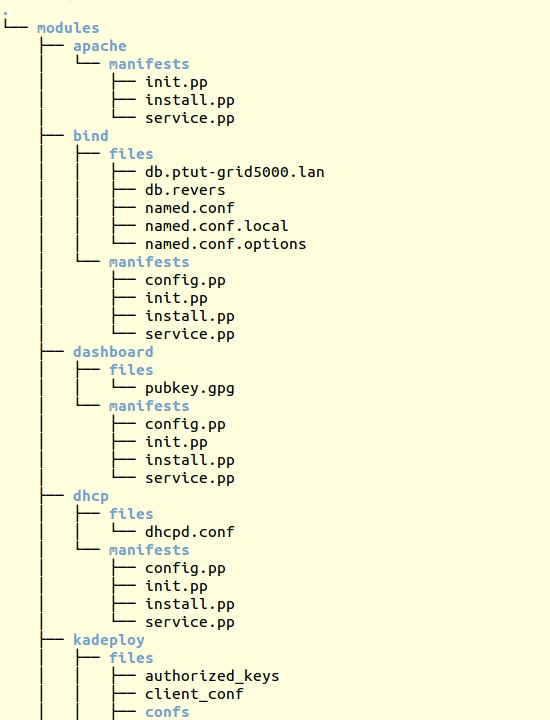
\includegraphics[scale=0.365]{Tree1.jpg}	
			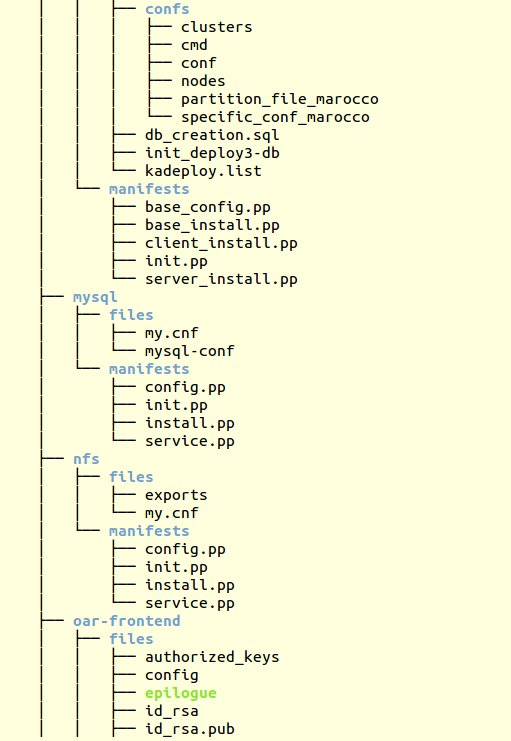
\includegraphics[scale=0.397]{Tree2.jpg}
			\label{Arborescence}
			\centering			
			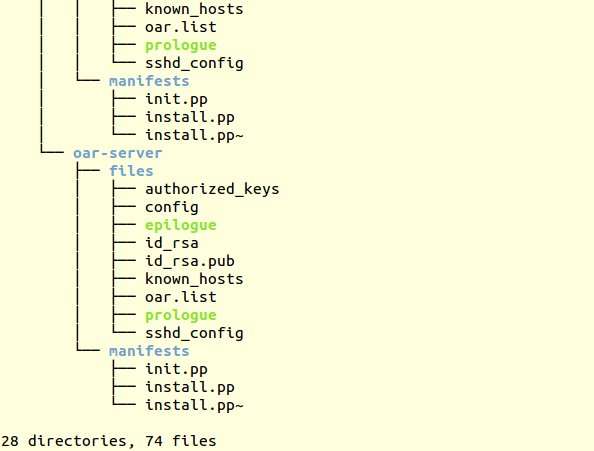
\includegraphics[scale=0.365]{Tree3.jpg}
			\caption{L'arborescence des modules.}	
			\label{Arbo2}
		\end{figure}
\newpage
			\subsection{Le logiciel OAR.}
			Comme expliqué plus haut, OAR se décompose ici en deux parties : le serveur et la frontend. Ces deux modules nécessitent un certain nombre de paramètres qui lui permettent de fonctionner :
				\begin{itemize}
					\item Une communication SSH qui permettent à la frontend de se connecter directement sur le serveur et inversement ;
					\item Le fichier de dép\^ot de logiciels d'OAR.
				\end{itemize}
				Nous copions donc l'intégralité des clés SSH créées pour l'occasion, ainsi que le fichier de configuration de notre utilisateur et le fichier de configuration du démon SSH.	
				L'ensemble de cette configuration, déployée à l'identique sur le frontend et le serveur, est définie par une classe située dans le fichier install.pp de chaque module OAR. 

			\subsubsection{Le module OAR-frontend.}
			Il est configuré par deux programmes : les fichiers prologue et epilogue. Par défaut, ils nécessitent absolument une configuration manuelle.
			\subsubsection{Le module OAR-server.}
		Le serveur OAR dépend activement d'une base de données, en l'occurence ici une base mysql. Cette base est configurée dans le fichier oar.conf, que nous allons copier depuis le maître Puppet vers le client.
		Deux autres fichiers de configuration sont nécesaires pour le serveur OAR. Il s'agit de : \begin{itemize}
		\item Monika.conf, qui permet de montrer les jobs soumis par la frontend au serveur ainsi que l'état de chaque noeud ;
		\item drawgantt.conf, qui permet de présenter les différentes tâches dans le temps suivant un Diagramme de Gantt.
\end{itemize}
Le serveur OAR nécessite également plusieurs autres services :
\begin{itemize}
\item un serveur Web du type apache2 sur la machine déployée ;
\item une base de données de type mysql ou postgre qui peut être sur une autre machine.
\end{itemize}

\end{document}
